\documentclass[12pt,letterpaper]{hmcpset}
\usepackage[margin=1in]{geometry}
\usepackage{graphicx}
\usepackage{enumitem} % enumerate
\usepackage{color} % hw6 specific, from tex hw source
% example usage of amssymb: $\mathbb{Z}$
% amsmath is loaded.
\newcommand{\remB}[1]{\textcolor{blue}{#1}}
\newcommand{\remR}[1]{\textcolor{red}{#1}}

% info for header block in upper right hand corner
\name{}
\class{Math 19 - 01}
\assignment{Homework \#6}
\duedate{10/11/2019}

\begin{document}

\problemlist{Homework \#6}

\begin{problem}[1]
  \textbf{(Average Value Theorem).} In HW 3 you showed that if $f$ is a positive continuous function on $[a,b]$ then there exists some $c \in (a,b)$ such that the area $A$ under the graph of $f$ satisfies $A = f(c) (b-a).$ Apply the Mean Value Theorem to the function $F(x) = \int_a^x f(t)\,dt$  to show that this property holds for any continuous function $f$ (not just positive) and that, in fact, the value $f(c)$ is given by  
  \begin{equation}
    f(c) = \frac{1}{b-a} \int_a^b f(t) \, dt.
    \label{boo}
  \end{equation}

  \noindent \textbf{Note:} The value $f(c)$ in \eqref{boo} is called \textit{the average value of $f$ on the interval $[a,b]$}. For a discrete set of values their average is the sum of values divided by the total number of values; here we have a continuum of values $f(x)$ for $x \in [a,b]$ and their average is the continuous sum of values $f(x)$ for $x \in [a,b]$ ($\int_a^b f(t) \, dt$) divided by the total number of $x$'s ($b-a$). 
\end{problem}
\begin{solution}
\end{solution}
\pagebreak

\begin{problem}[2]
  \begin{enumerate}[label=(\alph*)]
  \item Determine $F'\left( \sqrt{\frac{\pi}{4}}\right)$ if $F(x) = \displaystyle \int_0^{\sin x^2} \frac{1}{t} \ dt$.
  \item Determine  $f(4)$ if $\displaystyle \int_0^x f(t) \, dt = x\cos(\pi x).$ \\
    Hint for (b): The answer is not $\displaystyle \int_0^4 f(t) \,dt$.
  \end{enumerate}
\end{problem}
\begin{solution}
\end{solution}
\pagebreak

\begin{problem}[3]
  Consider $\displaystyle f(x) = \frac{\ln x}{x}$ for $x > 0$. 
  \begin{enumerate}[label=(\alph*)]
  \item Show $f$ has a global maximum at $e$. What is the maximum value of $f$? 
  \item Sketch a graph of the function $f$. 
  \item Since $e < \pi$ it follows from (a) that $\frac{\ln \pi}{\pi} < \frac{\ln e}{e}$. Use this to show $\pi^e < e^{\pi}$. 
  \end{enumerate}
\end{problem}
\begin{solution}
\end{solution}
\pagebreak

\begin{problem}[4]
(\textbf{Hyperbolic Trig functions}.)
The hyperbolic sine and cosine are important functions in many areas of science and engineering. They are defined by
$$\sinh x = \frac{e^x-e^{-x}}{2} = \frac{1}{2}e^x - \frac{1}{2} e^{-x}\qquad \text{ and } \qquad 
\cosh x = \frac{e^x+e^{-x}}{2} =\frac{1}{2}e^x + \frac{1}{2}e^{-x}.$$

\noindent 
\parbox{0.45\textwidth}{
\[ 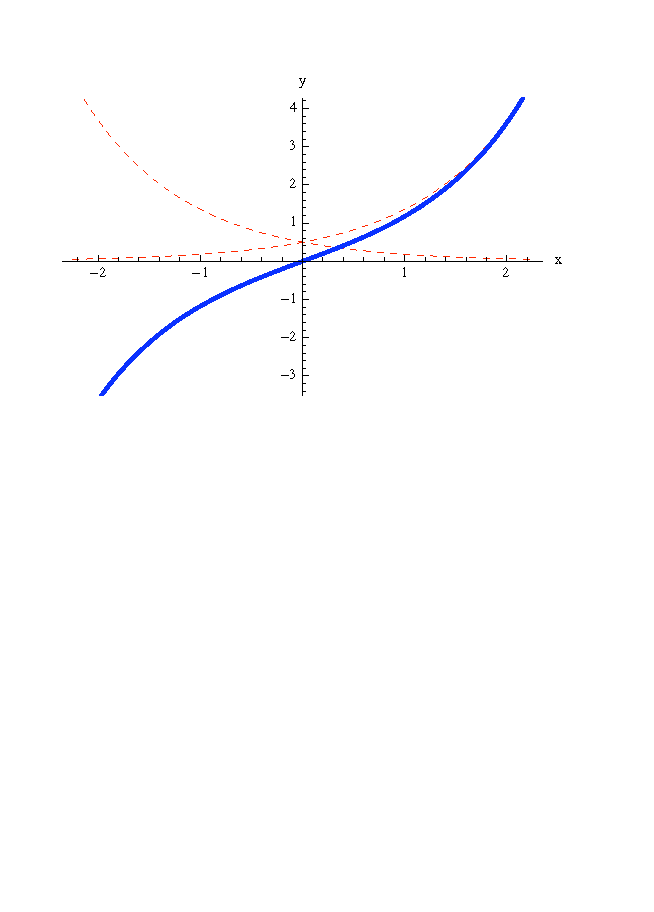
\includegraphics[width=0.425\textwidth]{assets/sinh}   \]
 \[  \remB{\sinh x} = \remR{\frac{e^x}{2} - \frac{e^{-x}}{2}}  \]
 }
 \parbox{0.45\textwidth}{
 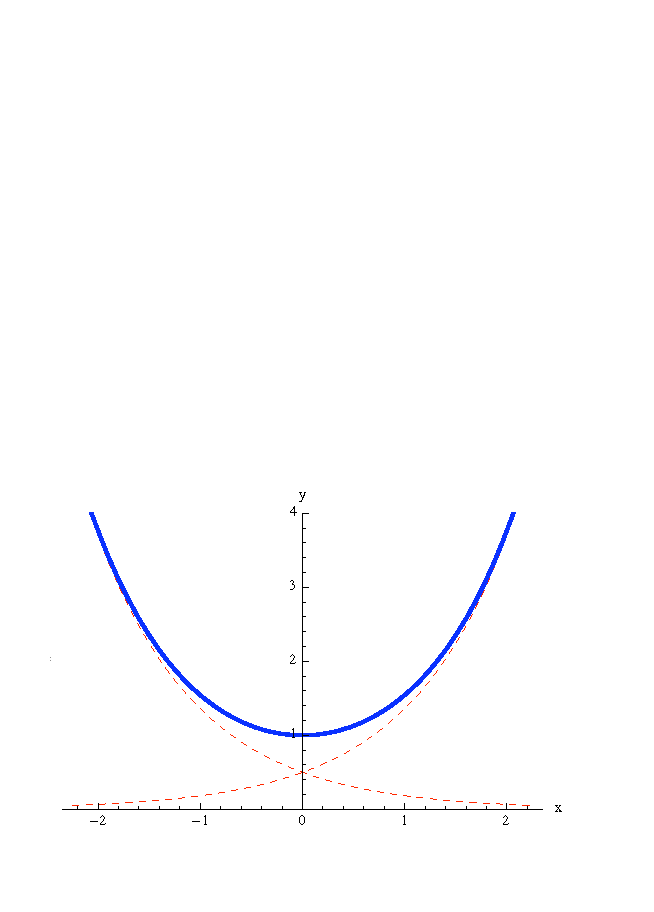
\includegraphics[width=0.425\textwidth]{assets/cosh} 
 \[  \remB{\cosh x} = \remR{\frac{e^x}{2} + \frac{e^{-x}}{2}} \]
 }
 
(dashed graphs are of $e^x/2$ and $e^{-x}/2$, $\sinh x$ is their difference, $\cosh x$ is their sum). 

The hyperbolic trig functions are not periodic, but they share many similar  properties to their periodic cousins $\sin x$ and $\cos x$.
\begin{enumerate}[label=(\alph*)]
\item Show that $\sinh 0 = 0$ and $\cosh 0 = 1$.
\item Show that $\sinh x$ is an odd function and $\cosh x$ is an even function.
\item Show that $\cosh^2 x - \sinh^2 x = 1$. 
\item Part (c) implies the set of points $(x,y) = (\cosh t, \sinh t)$ satisfy $x^2 - y^2 = 1$, an equation whose graph is a hyperbola. Do the points $(\cosh t, \sinh t)$ cover the entire hyperbola $x^2 - y^2 = 1$? Explain.  
\end{enumerate}
\end{problem}
\begin{solution}
\end{solution}
\newpage \phantom{long answer} \newpage

\begin{problem}[5]
The following figure illustrates another interesting connection between the circular trig functions sine and cosine and the hyperbolic trig functions sinh and cosh:
\[ 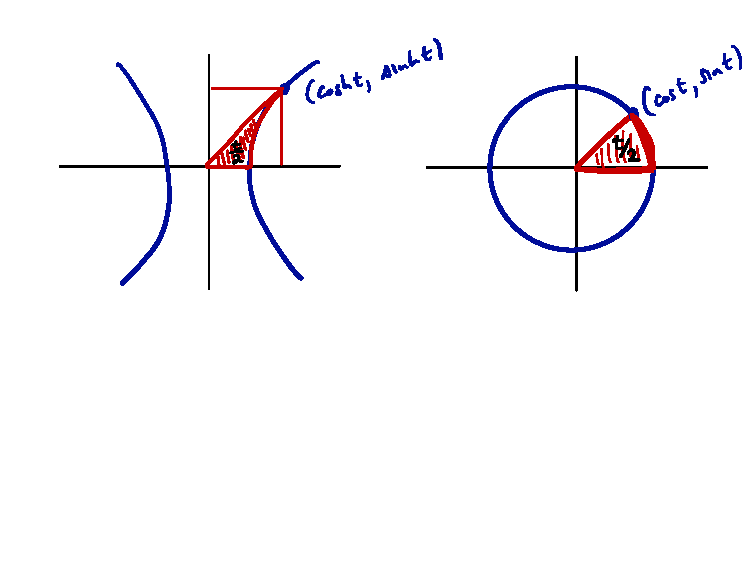
\includegraphics[width=0.75\textwidth]{assets/hyperboliccool2}  \]
In each case the area of the shaded region defined by $t$ is $t/2$. For the circle, the entire area is $\pi$ and the wedge has radian angle $t$, so the area is $A = \frac{t}{2\pi} \cdot \pi = \frac{t}{2}$. 
For the hyperbola, the shaded area can be realized as the area of the triangle defined by the points $(0,0), (\cosh t, 0), $ and $(\cosh t, \sinh t)$, less the area under the hyperbola from $x=1$ to $x=\cosh t$: 
\[ A(t) = \frac{1}{2} \cosh t \sinh t - \int_1^{\cosh t} \sqrt{x^2 - 1} \ dx  \]
\begin{enumerate}[label=(\alph*)]
\item Instead of computing this unfriendly integral for $A(t)$, first show that  $A'(t) = \frac{1}{2}$. 
\item Explain why part (a) implies $A(t) = \frac{t}{2}  + C$ for some constant $C$. 
\item Use the known value $A(0)$ to determine $C$ and therefore verify $A(t) = \frac{t}{2}$, as desired. 
\end{enumerate}
\end{problem}
\begin{solution}
\end{solution}
\pagebreak\phantom{long answer}\pagebreak

\begin{problem}[6]
\textbf{(Derivatives of Hyperbolic Trig Functions)}
\begin{enumerate}[label=(\alph*)]
\item Show that 
$$\frac{d}{dx} (\, \sinh x \,) = \cosh x \hskip 30 pt \frac{d}{dx} ( \, \cosh x \,) = \sinh x$$
\item Use the result of (a) to verify that  $y = \sinh x$ and $y = \cosh x$ each satisfy the differential equation
\begin{equation}
  y'' = y.
  \label{sh}
  \end{equation}
Similarly, verify that $y = \sin x$ and $y = \cos x$ each satisfy the differential equation
\begin{equation}
 y'' = -y.
   \label{sh2}
  \end{equation}
We will see in Math 82 that, in fact,  \textit{any} solution of \eqref{sh} has the form $y = c_1 \sinh x + c_2 \cosh x$ for some constants $c_1$ and $c_2$, and \textit{any} solution of \eqref{sh2} has the form $y = c_1 \sin x + c_2 \cos x$ for some constants $c_1$ and $c_2$. We say these functions form a ``basis" for the set of all solutions. 
\item One defines the hyperbolic tangent (read ``tanch") and hyperbolic secant (read ``setch") by 
$$\tanh x = \frac{\sinh x}{\cosh x} \qquad \text{ and } \qquad  {\rm sech}\ x = \frac{1}{\cosh x}. $$
Show that
$$\frac{d}{dx}\tanh x = {\rm sech}^2\, x\hskip 30 pt 
\frac{d}{dx} {\rm sech}\, x = -\tanh x\ {\rm sech}\ x.$$
\end{enumerate}
\end{problem}
\begin{solution}
\end{solution}





\end{document}
